\subsection{Description}\label{sec:prel:desc}

The dataset is composed of 46 different solutions at different radii. Each of
them is then composed of lists of several observables of different lengths
(varying from 15 to 21 entries each, as shown in \Cref{fig:prelim:length}).
\begin{figure}[htbp]
  \centering
  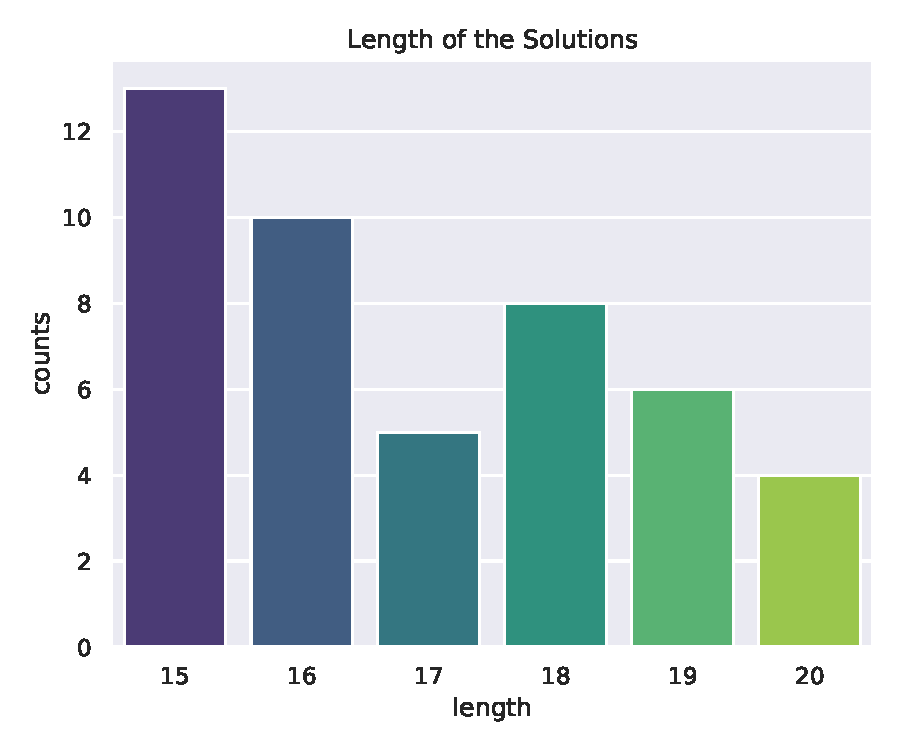
\includegraphics[width=0.4\textwidth]{img/length-solutions}
  \caption{Length of the solutions in the untidied dataset.}
  \label{fig:prelim:length}
\end{figure}
Every observable is characterised by its conformal weight (the \texttt{weight}
column in the dataset), its kind of ``oscillations'' (\texttt{type} variable,
categorical and ordered), its initialisation point (\texttt{init}) and the
truncation levels (from level 2 to level 18).
The objective of the analysis is the prediction of the extrapolation for the
level-$\infty$ truncation hosted in the \texttt{exp} variable of the dataset and which take 3 possible integer values in the range $[-1, 1]$.

\subsection{Input Preparation}\label{sec:prel:prep}

For the analysis we extract each entry of the lists and put it in separate
entry of the dataset: we first artificially insert a new variable labelling the
solution with a number from 0 to 45 and then flatten the dataset over the rows.
This way all columns hold only numerical variables which can be used for
different steps of the analysis.
The tidy dataset is composed of 778 samples over 22 columns (including the
newly created \texttt{solutions} variable).

We then look for duplicates inside the tidy dataset: rows which present exactly
the entries over all the columns, and exclude them from the analysis (we keep
only the first occurrence).
The final version of the dataset holds 732 samples and can be used for the
exploratory data analysis (EDA).
